\section{Prototyping}
This section will explain how important prototyping and sketching was in this project and how it helped in the preanalysis. \\\\
In this project a very big part have been prototyping and sketching. This was done to gather understanding about how the final designe would look like and how it could be improved further. The sketches was used to gather some information about how the \guardian{}s saw the design and if the design were right for them. The prototypes was improved, remade over and over because of the iterative workform. The most important part of the overall design happened in the sketching and prototyping phase, all activities and their screens was made this way. \\
A late version of a prototype was represented to the \guardian{}s from \egebakken{}. This was a papir-prototype and represented two things about the product: How the screens was ment to be implemented, designed and how the flow in the program was going to be. It was designed so that buttons could be seen and when pressed on a button it linked to a new page of papir. This was done so the \guardian{}s could try out the program even before it was made and talk about what they had in mind about the overall design of the launcher.
This was done so the \guardian{}s could come with feedback on which screens or activities should be changed as it was important to hear what the costumer had to say. It was also done so it was possible to check out how the flow was and if it was good enough or had to be improved further. An overview of this prototype can be seen in \autoref{fig:first-prototype}

\begin{figure}[h!]
	\centering
	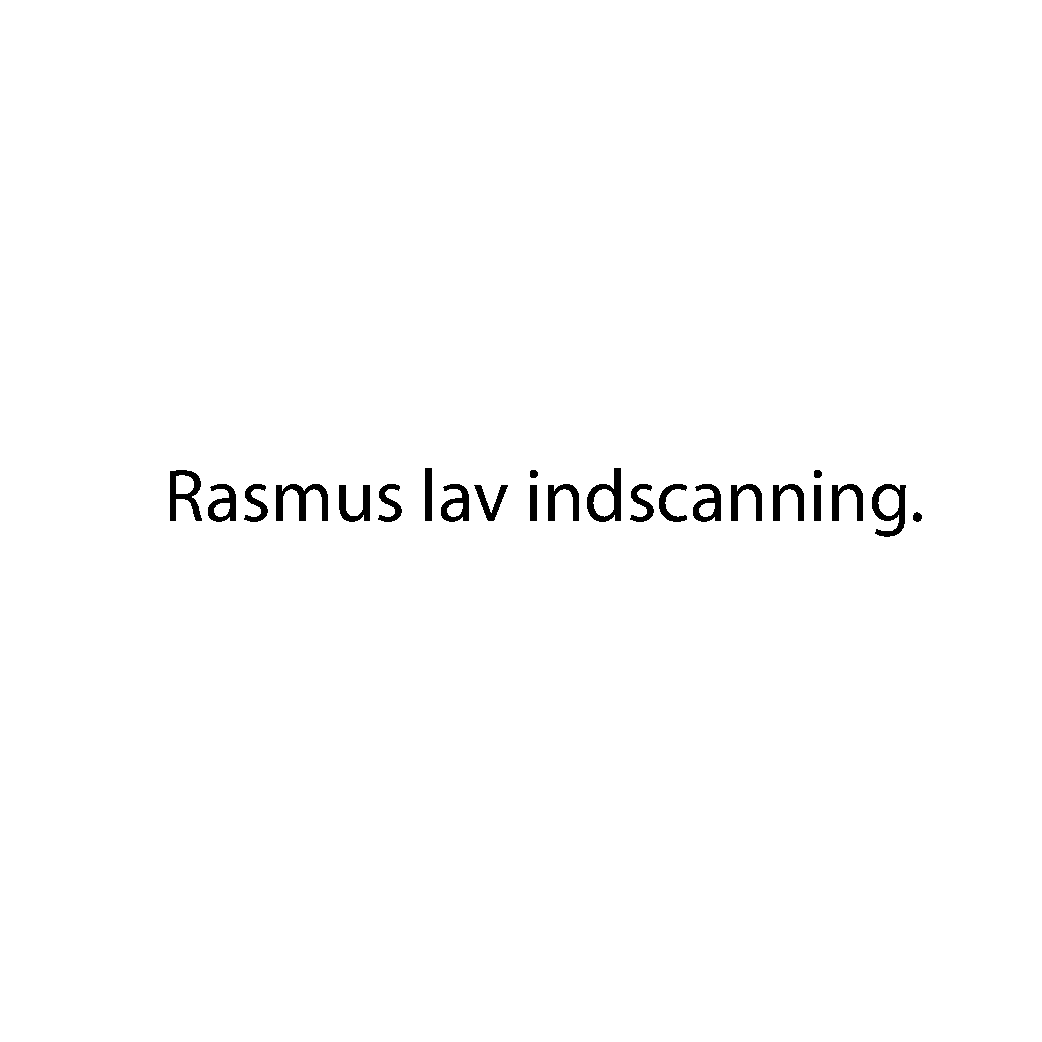
\includegraphics[scale=0.5]{gfx/first-prototype.pdf}
	\caption{Activity overview page from one of the first prototypes.}
	\label{fig:first-prototype}
\end{figure}

